\documentclass[letterpaper,12pt,twoside,]{pinp}

%% Some pieces required from the pandoc template
\providecommand{\tightlist}{%
  \setlength{\itemsep}{0pt}\setlength{\parskip}{0pt}}

% Use the lineno option to display guide line numbers if required.
% Note that the use of elements such as single-column equations
% may affect the guide line number alignment.

\usepackage[T1]{fontenc}
\usepackage[utf8]{inputenc}

% pinp change: the geometry package layout settings need to be set here, not in pinp.cls
\geometry{layoutsize={0.95588\paperwidth,0.98864\paperheight},%
  layouthoffset=0.02206\paperwidth, layoutvoffset=0.00568\paperheight}

\definecolor{pinpblue}{HTML}{185FAF}  % imagecolorpicker on blue for new R logo
\definecolor{pnasbluetext}{RGB}{101,0,0} %


\usepackage{subfig}

\title{Assignment 3 - Data Visualization. Due October 3, 11:59pm 2021}

\author[a]{EPIB607 - Inferential Statistics}

  \affil[a]{Fall 2021, McGill University}

\setcounter{secnumdepth}{5}

% Please give the surname of the lead author for the running footer
\leadauthor{EPIB607}

% Keywords are not mandatory, but authors are strongly encouraged to provide them. If provided, please include two to five keywords, separated by the pipe symbol, e.g:
 

\begin{abstract}
All questions are to be answered in an R Markdown document using the
provided template and compiled to a pdf document. You are free to choose
any function from any package to complete the assignment. Concise
answers will be rewarded. Be brief and to the point. Each question is
worth 25 points. Label your graphs appropriately with proper titles and
axis labels. Justify your answers. You may compile your reoport to pdf
or to HTML. If you compile to HTML, then you must print the resulting
HTML to pdf. Please submit the compiled pdf report to Crowdmark. You
must also submit your code to Crowdmark. If you use the template, the
code from your assignment will automatically appear at the end. Upload
this code to Q5 in Crowdmark. You can upload a single pdf to Crowdmark,
and then select the pages for a given question. See
\url{https://crowdmark.com/help/} for details.
\end{abstract}

\dates{This version was compiled on \today} 

% initially we use doi so keep for backwards compatibility
% new name is doi_footer

\pinpfootercontents{Assignment 3}

\begin{document}

% Optional adjustment to line up main text (after abstract) of first page with line numbers, when using both lineno and twocolumn options.
% You should only change this length when you've finalised the article contents.
\verticaladjustment{-2pt}

\maketitle
\thispagestyle{firststyle}
\ifthenelse{\boolean{shortarticle}}{\ifthenelse{\boolean{singlecolumn}}{\abscontentformatted}{\abscontent}}{}

% If your first paragraph (i.e. with the \dropcap) contains a list environment (quote, quotation, theorem, definition, enumerate, itemize...), the line after the list may have some extra indentation. If this is the case, add \parshape=0 to the end of the list environment.


\hypertarget{template}{%
\section*{Template}\label{template}}
\addcontentsline{toc}{section}{Template}

Please use the \texttt{.Rmd} template for Assignment 3 which is
available on myCourses.

\hypertarget{points-mask-mandates-in-kansas}{%
\section{(25 points) Mask mandates in
Kansas}\label{points-mask-mandates-in-kansas}}

This question is based on the article
\href{https://www.kansas.com/news/politics-government/article244959870.html}{\emph{Kansas
began requiring masks, then virus cases dropped. Weeks later, `the data
is solid'}}. In a short press conference, Dr.~Lee Norman presents a
figure which is reproduced here in Figure \ref{fig:fig1}.

\begin{enumerate}
\def\labelenumi{\alph{enumi})}
\tightlist
\item
  (5 points) What does this graph make it appear is happening? What
  would your conclusion be about the importance of a mask mandate?\\
\item
  (5 points) Provide the column names of the tidy dataset that would
  have been used to create Figure \ref{fig:fig1}. For each column, name
  the aesthetic its being mapped onto.\\
\item
  (10 points) Using the data from Figure \ref{fig:fig1}, create an
  alternative visualization and interpret the graph. Be sure to label
  your axes and provide a descriptive title.\\
\item
  (5 points) Comment on the differences between Figure \ref{fig:fig1}
  and the graph you created in part b). Does the conclusion you
  described from part a) still hold ?
\end{enumerate}

\begin{figure}[H]

{\centering 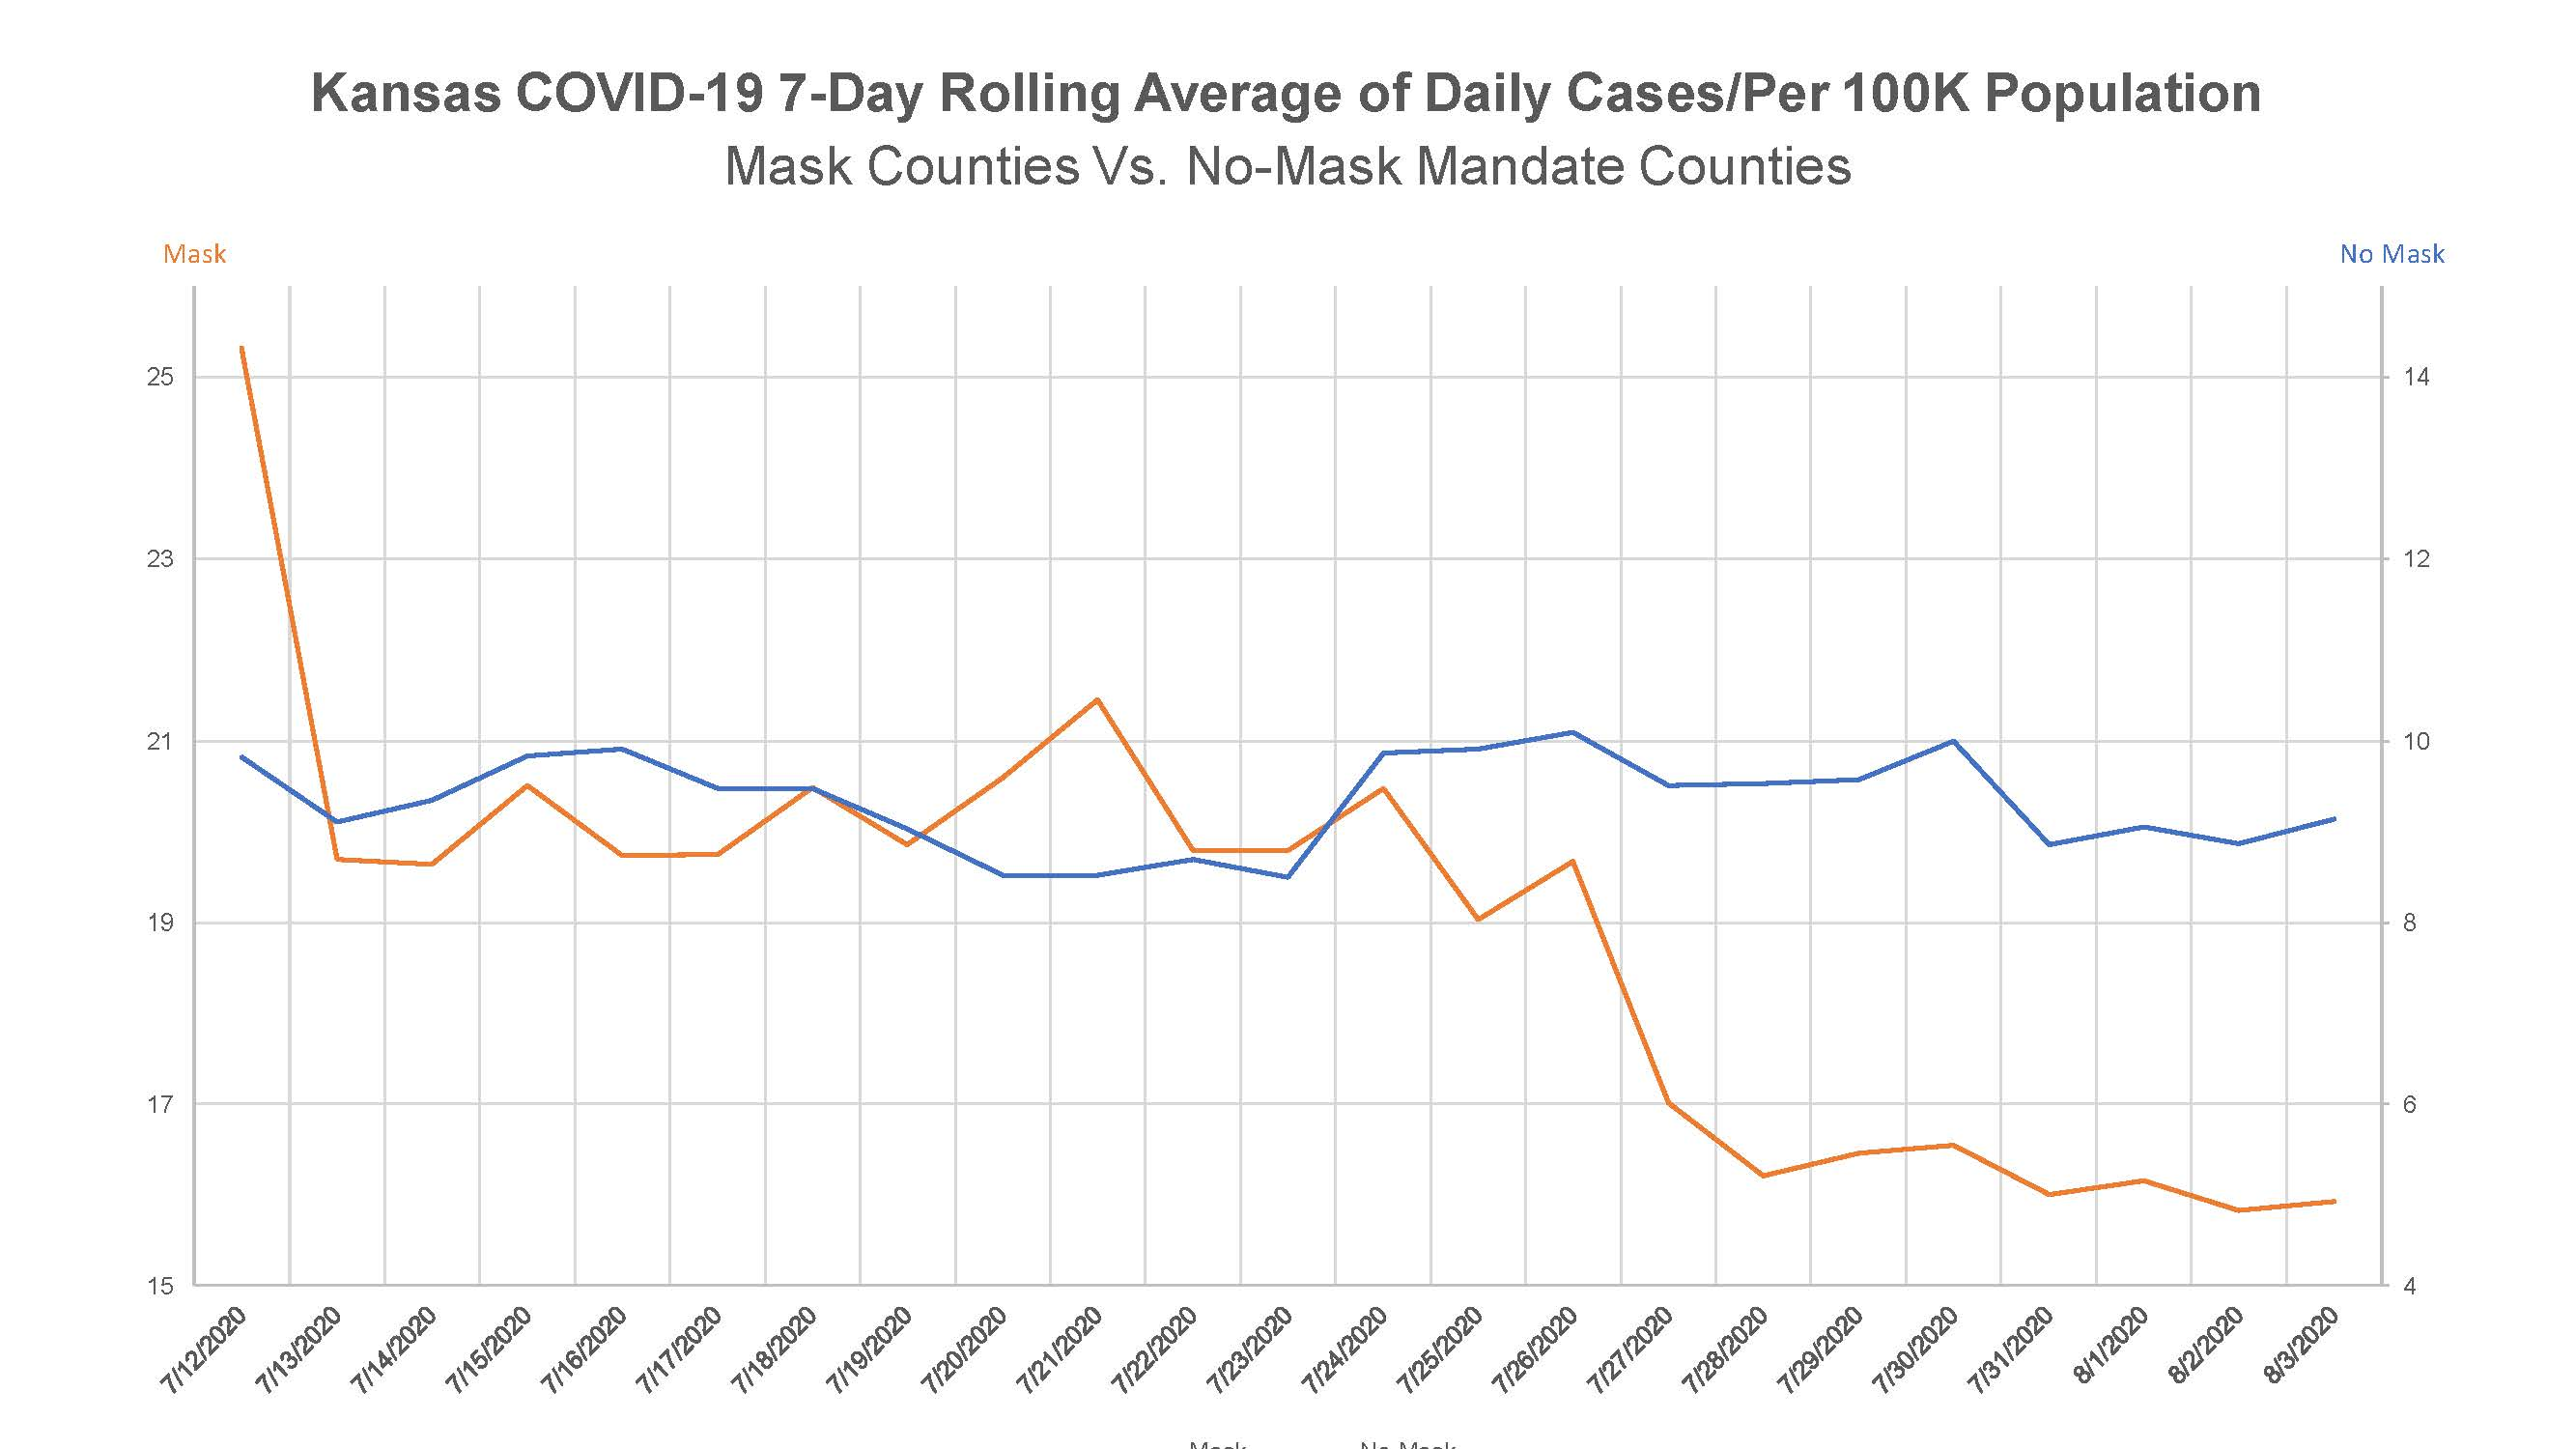
\includegraphics[width=0.99\textwidth]{/home/sahir/git_repositories/epib607/inst/assignments/a3/fig1} 

}

\caption{Kansas COVID-19 7-Day rolling average of cases per 100k.}\label{fig:fig1}
\end{figure}

\newpage

\hypertarget{points-are-covid-cases-decreasing-over-time-in-georgia}{%
\section{(25 points) Are Covid cases decreasing over time in
Georgia?}\label{points-are-covid-cases-decreasing-over-time-in-georgia}}

This question is based on the data presented by the
\href{https://www.ajc.com/news/state--regional-govt--politics/just-cuckoo-state-latest-data-mishap-causes-critics-cry-foul/182PpUvUX9XEF8vO11NVGO/}{Georgia
Department of Public Health} and shown in Figure \ref{fig:fig2}:

\begin{enumerate}
\def\labelenumi{\alph{enumi})}
\tightlist
\item
  (5 points) List the mappings of variables onto visual cues. What does
  this graph make it appear is happening? Is this a good visualization -
  why or why not?\\
\item
  (10 points) The data in the file \texttt{georgiaCounties.csv} contains
  daily COVID19 data for the 5 counties of interest in Georgia. In
  addition to \texttt{date}, \texttt{state}, \texttt{county},
  \texttt{population}, \texttt{daily\_cases} and \texttt{daily\_deaths}
  you are given \texttt{cases} which represents the cumulative number of
  cases, \texttt{deaths} represents the cumulative number of deaths, and
  \texttt{fips} which is the
  \href{https://transition.fcc.gov/oet/info/maps/census/fips/fips.txt}{Federal
  Information Processing System} codes for counties. The data can be
  read into \texttt{R} using the code shown below. Using this data,
  create an alternative version of Figure \ref{fig:fig2} and interpret
  the graph. Be sure to label your axes and provide a descriptive title.
\end{enumerate}

\begin{Shaded}
\begin{Highlighting}[]
\NormalTok{georgia }\OtherTok{\textless{}{-}}\NormalTok{ readr}\SpecialCharTok{::}\FunctionTok{read\_csv}\NormalTok{(here}\SpecialCharTok{::}\FunctionTok{here}\NormalTok{(}\StringTok{"georgiaCounties.csv"}\NormalTok{),}
                           \AttributeTok{col\_types =} \FunctionTok{c}\NormalTok{(}\StringTok{"Dfffddddd"}\NormalTok{))}
\end{Highlighting}
\end{Shaded}

\begin{enumerate}
\def\labelenumi{\alph{enumi})}
\setcounter{enumi}{2}
\tightlist
\item
  (5 points) Comment on the differences between Figure \ref{fig:fig2}
  and the graph you created in part b). Does the conclusion you
  described from part a) still hold ?\\
\item
  (5 points) Plot the data for a longer time horizon and comment on any
  patterns you see. Contrast this with Figure \ref{fig:fig2} and the
  figure you created in part b.
\end{enumerate}

\begin{figure}

{\centering 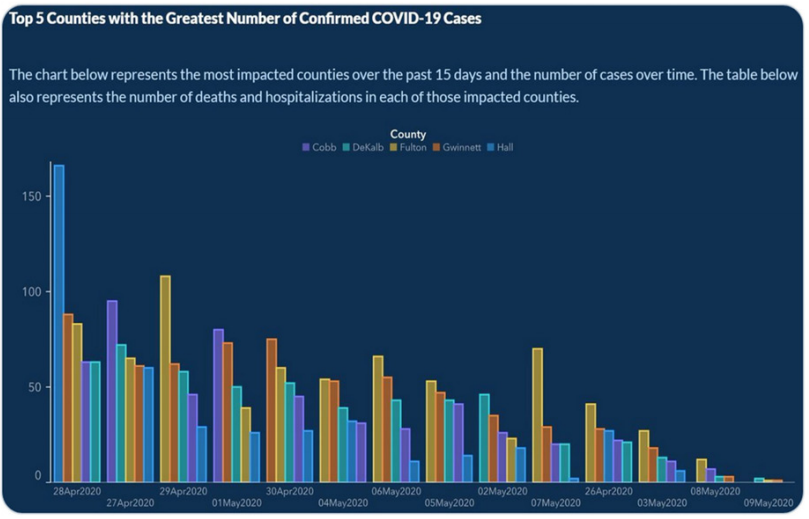
\includegraphics[width=0.99\textwidth]{/home/sahir/git_repositories/epib607/inst/assignments/a3/fig2} 

}

\caption{Georgia Department of Public Health Figure.}\label{fig:fig2}
\end{figure}

\newpage

\newpage

\hypertarget{points-food-in-america}{%
\section{(25 points) Food in America}\label{points-food-in-america}}

Vox published a list of
\href{http://www.vox.com/a/explain-food-america}{Charts that explain
food in America}. There are 40 maps, charts, and graphs that show where
our food and drink comes from and how we eat it.

\begin{enumerate}
\def\labelenumi{\alph{enumi})}
\tightlist
\item
  (20 points, 10 for best and 10 for least favorite) Pick your best and
  least favorite graphic, and briefly explain why using the taxonomy we
  learned in class (Sections
  \href{https://sahirbhatnagar.com/EPIB607/aesthetic-mapping.html}{2},
  \href{https://sahirbhatnagar.com/EPIB607/coordinate-systems-axes.html}{3}
  and \href{https://sahirbhatnagar.com/EPIB607/color-basics.html}{5})
  (e.g.~visual cues being used, one-to-one mapping, appropriate use of
  coordinate systems and color scales). Provide a link to each figure.
  For example, this link:
  \href{https://www.vox.com/a/explain-food-america\#list-21}{Figure 18}
  was created using the following code:
  \texttt{{[}Figure\ 18{]}(https://www.vox.com/a/explain-food-america\#list-21)}
\item
  (5 points) For either of the two graphs you chose in part a),
  \textbf{describe} an alternative version and explain its advantages
  over the original. You do not need to actually create the figure.
\end{enumerate}

\newpage

\hypertarget{points-geometries-in-ggplot2}{%
\section{(25 points) Geometries in
ggplot2}\label{points-geometries-in-ggplot2}}

\begin{enumerate}
\def\labelenumi{\alph{enumi})}
\item
  (5 points) In Figure
  \href{https://sahirbhatnagar.com/EPIB607/ggplot2-package-for-plots.html\#fig:03-make-a-plot-8}{4.6}
  of the course website notes, we plotted life expectancy vs.~GDP per
  capita from the gapminder data with point and smooth geometries. What
  happens when you put the \texttt{geom\_smooth()} function before
  \texttt{geom\_point()} instead of after it? What does this tell you
  about how the plot is drawn? Think about how this might be useful when
  drawing plots.
\item
  (2.5 points) What happens if you map \texttt{color} to \texttt{year}
  instead of \texttt{continent}? Explain this behavior.
\item
  (2.5 points) Instead of mapping \texttt{color\ =\ year}, what happens
  if you try \texttt{color\ =\ factor(year)}? Explain this behavior.
\item
  (5 points) The \texttt{Oxboys} dataset, from the \texttt{nlme} package
  records the heights (\texttt{height}) and centered ages (\texttt{age})
  of 26 boys (\texttt{Subject}), measured on nine occasions
  (\texttt{Occasion}). Figure \ref{fig:ggplot} is a line plot of height
  vs.~age. Is this an appropriate visualization of the data? If yes,
  interpret the figure. If no, explain what is wrong. Create an
  alternative visualization by modifying the code below and interpret
  this graph.
\end{enumerate}

\begin{Shaded}
\begin{Highlighting}[]
\FunctionTok{data}\NormalTok{(Oxboys, }\AttributeTok{package =} \StringTok{"nlme"}\NormalTok{)}
\NormalTok{p }\OtherTok{\textless{}{-}} \FunctionTok{ggplot}\NormalTok{(}\AttributeTok{data =}\NormalTok{ Oxboys, }\FunctionTok{aes}\NormalTok{(}\AttributeTok{x =}\NormalTok{ age, }\AttributeTok{y =}\NormalTok{ height))}
\NormalTok{p }\SpecialCharTok{+} \FunctionTok{geom\_line}\NormalTok{()}
\end{Highlighting}
\end{Shaded}

\begin{figure}[H]

{\centering 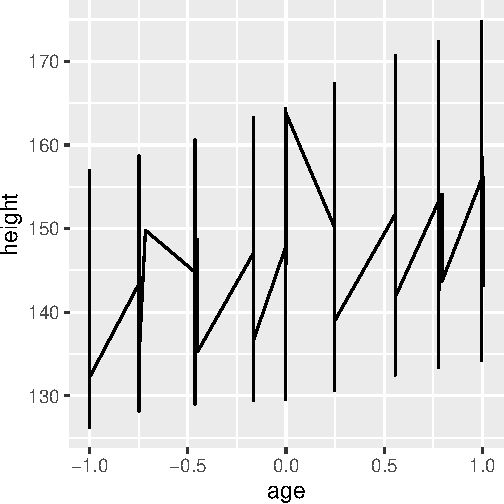
\includegraphics{a3-data-summary_files/figure-latex/ggplot-1} 

}

\caption{Height vs age for the Oxboys data.}\label{fig:ggplot}
\end{figure}

\begin{enumerate}
\def\labelenumi{\alph{enumi})}
\setcounter{enumi}{4}
\tightlist
\item
  (10 points, 5 each) Figure \ref{fig:gg2} illustrates the difference
  between mapping continuous and discrete colours to a line and code is
  given below to reproduce these plots.

  \begin{enumerate}
  \def\labelenumii{\roman{enumii})}
  \tightlist
  \item
    Explain the purpose of the \texttt{aes(group\ =\ 1)} code.\\
  \item
    What's the difference between \texttt{aes(group\ =\ 1)} and
    \texttt{aes(group\ =\ 2)}? Why?
  \end{enumerate}
\end{enumerate}

\begin{Shaded}
\begin{Highlighting}[]
\NormalTok{df }\OtherTok{\textless{}{-}} \FunctionTok{data.frame}\NormalTok{(}\AttributeTok{x =} \DecValTok{1}\SpecialCharTok{:}\DecValTok{3}\NormalTok{, }\AttributeTok{y =} \DecValTok{1}\SpecialCharTok{:}\DecValTok{3}\NormalTok{, }\AttributeTok{colour =} \FunctionTok{c}\NormalTok{(}\DecValTok{1}\NormalTok{,}\DecValTok{3}\NormalTok{,}\DecValTok{5}\NormalTok{))}

\FunctionTok{ggplot}\NormalTok{(df, }\FunctionTok{aes}\NormalTok{(x, y, }\AttributeTok{colour =} \FunctionTok{factor}\NormalTok{(colour))) }\SpecialCharTok{+} 
  \FunctionTok{geom\_line}\NormalTok{(}\FunctionTok{aes}\NormalTok{(}\AttributeTok{group =} \DecValTok{1}\NormalTok{), }\AttributeTok{size =} \DecValTok{2}\NormalTok{) }\SpecialCharTok{+}
  \FunctionTok{geom\_point}\NormalTok{(}\AttributeTok{size =} \DecValTok{5}\NormalTok{) }\SpecialCharTok{+} \FunctionTok{labs}\NormalTok{(}\AttributeTok{title =} \StringTok{"Discrete example"}\NormalTok{)}

\FunctionTok{ggplot}\NormalTok{(df, }\FunctionTok{aes}\NormalTok{(x, y, }\AttributeTok{colour =}\NormalTok{ colour)) }\SpecialCharTok{+} 
  \FunctionTok{geom\_line}\NormalTok{(}\FunctionTok{aes}\NormalTok{(}\AttributeTok{group =} \DecValTok{1}\NormalTok{), }\AttributeTok{size =} \DecValTok{2}\NormalTok{) }\SpecialCharTok{+}
  \FunctionTok{geom\_point}\NormalTok{(}\AttributeTok{size =} \DecValTok{5}\NormalTok{) }\SpecialCharTok{+} \FunctionTok{labs}\NormalTok{(}\AttributeTok{title =} \StringTok{"Continuous example"}\NormalTok{)}
\end{Highlighting}
\end{Shaded}

\begin{figure}

{\centering \subfloat[Discrete example.\label{fig:gg2-1}]{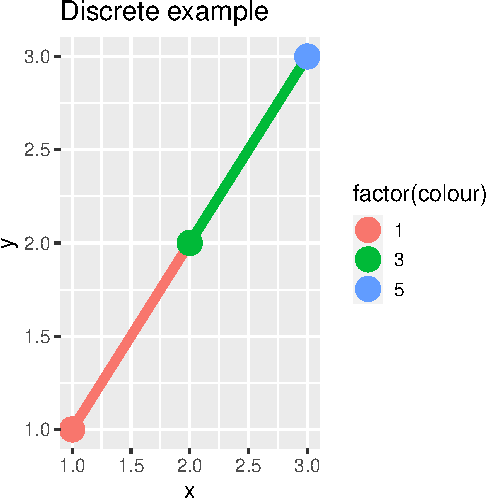
\includegraphics{a3-data-summary_files/figure-latex/gg2-1} }\subfloat[Continuous example\label{fig:gg2-2}]{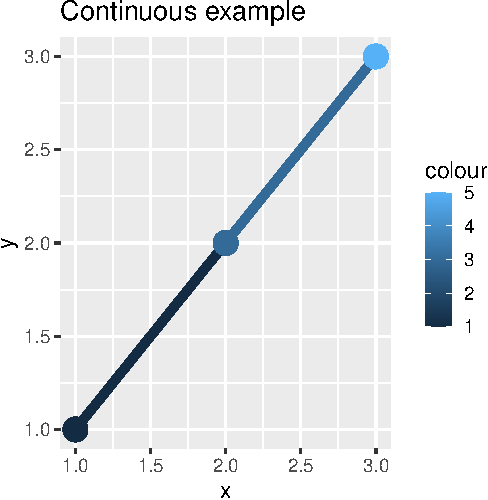
\includegraphics{a3-data-summary_files/figure-latex/gg2-2} }

}

\caption{Difference between mapping continuous and discrete colours to a line}\label{fig:gg2}
\end{figure}

%\showmatmethods


\bibliography{pinp}
\bibliographystyle{jss}



\end{document}
